
\begin{abstract}

Simulating the cloud from the client point of view.

Assessment of the impact of different metrics.

Recommendations for using cloud simulators.

WARNING: figures in text might not be up to date.

\end{abstract}

\section{Introduction}

The  problem   of  allocating   cloud  resources   in  performant,   robust  and
energy-efficient ways is  of paramount importance in today's  usage of computing
infrastructures. Cloud resources  proposed to clients as \ac{iaas}  open a large
field of  investigation regarding how automatic  tools can hepl users  to better
provision the  resources and  schedule their computation  or storage  tasks with
regard to the trade-off between rental  cost and performance.  Indeed it rapidly
becomes  very difficult  for  users  to manually  handle  the provisionning  and
scheduling  decisions  when the  workloads  involve  numerous tasks,  which  are
potentially dependent on  others -- and such complex workloads  are the focus in
this paper. In the last decade a  number of research papers have contributed new
allocation techniques to address this issue.  A pitfall of research on \ac{iaas}
lies in the  validation of the models and algorithms  proposed, as validation on
actual  clouds  requires  infrastructures  that  are difficult  to  set  up  for
individual researchers.  As a consequence,  many researchers evaluate their work
through simulation. A number of simulators  have been developed for that purpose
as reviewed in the related work  section hereafter.  They are typically based on
discrete-event simulation,  using models  for each  elementary component  of the
infrastructure,  which  are then  composed  to  simulate  the whole  system  and
applications running on it.

However, such  an \textit{ab  initio} construction  poses a  significant problem
regarding  the  calibration  and  validation   of  the  composed  model  against
real-world measurements. We  show in this paper that a  precise modeling of each
component  may not  be sufficient  to yield  accurate predictions  of the  whole
system's  behavior.   Yet,  from  the client-side  (or  equivalently,  from  the
application perspective),  the validaty of  the simulation is  evaluated against
macros-metrics, such  as the  makespan and  the rental  cost of  the application
executions. It means that the interactions betweens all components must be taken
into account in the simulation, including the lower level components such as the
network  sharing or  the higher  level components  such as  the scheduler.   For
instance, a decision which starts simultaneously  a large number of \acp{vm} may
result in trashing~\cite{MarshallKF10} affecting the expected performance.

This work's  objective is  to study how  an actual cloud  setup behavior  can be
predicted through simulation on practical use-cases.   To that end, we propose a
simulation framework called SCHiaaS\footnote{SCHIaaS stands for \emph{Simulation
    of Cloud, Hypervisor and IaaS}.}  which specializes in IaaS clouds modeling.
This  is an  extension  to the  SimGrid simulation  toolkit~\cite{CasanovaLQ08},
which  provides  in particular  the  discrete  event  simulator engine  and  the
operating-system level operations (e.g  messaging, virtual machines management).
Using SCHIaaS,  we focus in  this article on  the modeling of  a cloud-brokering
system. This  client-side broker, on behalf  on its users, makes  scheduling and
provisioning   decisions,   and   automates   jobs'  execution   on   the   real
infrastructure. We have  used this brokering system to experiment  the impact of
scheduling and  provisioning policies  when running two  scientific applications
using  cloud computing  resources.  The  exact  setting for  this experiment  is
described in Section~\ref{sc:context}. The  question that this article addresses
is:  can this  brokering  system  be modeled  and  predicted accurately  through
simulation? We have collected numerous  execution logs traces when running these
scientific applications through the broker, and these provide us with a valuable
basis to validate our candidate simulation model.

The broker,  called \textit{Schlouder}~\cite{Michon17},  has been  developped by
our   team,  and   our  effort   to   build  a   simulator  of   it  is   called
\textit{SimSchlouder}.  This  co-development approach makes this  study original
as allmost all the previous cloud  simulation software proposed have put forward
first the  design of their software  library, leaving the precise  validation to
fure  experiments.  By  contrast, we  have been  able to  add all  the necessary
instrumentation in  the broker and  in the simulator  to help us  understand how
accurate were the predictions for  indivual simulated components, especially for
higher  level components  such as  the modeling  of \ac{vm}  boot times  and the
scheduling policies. This continuous analysis has allowed us to fine tune the
simulation software. 

% ------- à recaser -----
%At the lower level,
% we rely on the discrete event simulation toolkit SimGrid~\cite{CasanovaLQ08} for
% which   validation  results   regarding  accuracy   have  been   published  (e.g
%\cite{StanisicTLVM15,VelhoSCL13}). 

This  paper's  contributions  is  therefor  twofold. First,  we  propose  a  new
simulation  tool extending  SimGrid with  an  interface capable  of modeling  of
\ac{iaas} clouds by providing a new  interface for that field. This interface is
publicly  available as  open-source  software.  Above  this  interface, we  also
developed  SimSchlouder to  demonstrate how  a client-side  cloud broker  can be
modeled using this interface.
%
Secondly,  as we  advocate that  a precise  assessment of  simulation should  be
carried out  against real execution figures  to better understand the  limits of
simulation  applicability, we  make an  in-depth  analysis of  the factors  that
impact the simulation  accuracy, and in this regard go  further than the related
works. We analyze the sensitivity of  several parameters, among which the impact
of the  job submission management overheads,  the effect of inaccuracies  in the
job execution times specified  by the user, or the boot time  of VMs.  The study
is  carried out  on several  use  cases which  comprise two  different types  of
applications (workflow and  bag-of-tasks), with several size  instances for each
of them, and each application operated  on two different types of infrastructure
(private and public).


The paper is  organized as follows. We first present  the related work regarding
simulation in  Section~\ref{sc:relwork}.  Section \ref{sc:schiaas}  presents the
design of  SCHIaaS.  Section~\ref{sc:context}  describes the  system we  seek to
simulate),  which  includes the  cloud  management  system Schlouder,  the  real
platforms  on which  experiments are  run, and  the applications  that serve  as
test-cases. The last section presents the simulation. It first sketches the main
design issues for  modeling Schlouder. The second part is  a thorough evaluation
of  the  simulation  accuracy  against real  observations  on  the  applications
test-cases  presented  earlier.


%-------------------------- R E L .  W O R K -----------------------------------
\section{Related Work}
\label{sc:relwork}

In the  past decade, a number  of research works have  proposed simulation tools
for clouds. Some of them have a longer history as they build upon the experience
of researchers in  the simulation of computing grids. Most  cloud simulators are
based on \ac{des}.   In \aclp{des} the simulation is a  serie of events changing
the state of  the simulated system.  For  instance, events can be  the start (or
end) of  computations or of  communications.  The  simulator will jump  from one
event to the  next, updating the times  of upcoming events to  reflect the state
change in  the simulation.   Such \ac{des}-based simulators  require at  least a
platform   specification  and   an   application   description.   The   platform
specification describes both the physical nature of the cloud, e.g.~machines and
networks,  and the  management rules,  e.g.~\ac{vm} placement  and availability.
Depending on the simulator, the platform  specification can be done through user
code,  as   in  CloudSim~\cite{cloudsim}   for  example,  or   through  platform
description  files,  as  is  mostly the  case  in  SimGrid~\cite{simgrid}.   The
application description consists  in a set of computing  and communicating jobs,
often described  as an amount  of computation  or communication to  perform. The
simulator computes their  duration based on the platform  specification, and its
CPU and  network models.  An alternative  approach is to directly  input the job
durations extrapolated from actual execution traces.


The available  cloud \acp{des} can  be divided in  two categories. In  the first
category are  the simulators  dedicated to  study the  clouds from  the provider
point-of-view, whose purpose  is to help evaluating the design  decisions of the
datacenter. Examples  of such simulators are  MDCSim~\cite{MDCSim}, which offers
specific  and precise  models for  low-level components  including network  (e.g
InfiniBand or  Gigabit ethernet),  operating system kernel  and disks.   It also
offers a model  for energy consumption. However, the cloud  client activity that
can be  modeled is restricted  to web-servers, application-servers  or data-base
applications.   GreenCloud~\cite{greencloud} follows  the  same  purpose with  a
string  focus  on  energy  consumption  of cloud's  network  apparatus  using  a
packet-level  simulation  for  network  communications  (NS2).   In  the  second
category  are the  simulators  targeting the  whole  cloud ecosystem,  including
client activity. In this category, CloudSim~\cite{cloudsim} (originally stemming
from  GridSim) is  the most  broadly used  simulator in  academic research.   It
offers   simplified   models   regarding    network   communications,   CPU   or
disks. However, it is easily extensible  and serves as the underlying simulation
engine   in   a   number   of    projects   (e.g   \cite{Cai17},   see   section
\ref{sc:relwork-stochastic}).  Simgrid~\cite{simgrid} is the other long-standing
project,  which  when used  in  conjunction  with  the SchIaaS  cloud  interface
provides  similar  functionnalities  as   CloudSim.   Among  the  other  related
projects, are iCanCloud~\cite{iCanCloud} proposed  to address scalability issues
encountered  with  CloudSim  (written  in  Java) for  the  simulation  of  large
use-cases.  Most recently,  PICS~\cite{pics} has  been proposed  to specifically
evaluate simulation of  public clouds.  The configuration of  the simulator uses
only parameters  that can be  measured by the  cloud client, namely  inbound and
outbound  network  bandwidths,  average  CPU  power,  \ac{vm}  boot  times,  and
scale-in/scale-out policies. The  data center is therefore seen as  a black box,
for which  no detailed  description of  the hardware  setting is  required.  The
validation study  of PICS  under a  variety of use  cases has  nonetheless shown
accurate predictions.

At the core of DES is the solver.  The solver considers the states of the system
generated  by the  platform and  previous events  to compute  the timing  of the
future events. In most cases,  simulators have a \emph{bottom-up} approach: the
modeling concerns  low-level components  (machines, networks,  storage devices),
and  from  their  interactions  emerge the  high-level  behaviours.  Working  on
disjoint low level components make it easier  to tune the precision of the model
to the wanted accuracy or speed trade-off.

%------- modifier : c'était pour introduire le stochastique
\textbf{FIXME: next paragraph to be adapted depending on wether stochastic
  simulation is mentioned.}
However, when the simulated system is subject to variability, it is difficult to
establish  the  validity of  simulation  results  formally. Indeed,  given  some
defined inputs, a DES outputs a single deterministic result, while a real system
will output  slightly different results  at each repeated execution.   Hence, in
practice  the simulation  is informally  regarded as  valid if  its results  are
``close'' to one or  some of the real observations.  Notice  however that in the
field  of grid  or cloud  computing, published  results in  terms of  validation
against real settings are scarce relatively to the number of projects.



\section{SCHIaaS}
\label{sc:schiaas}

\subsection{Overview}
The first contribution of this paper is the simulation framework called SCHIaaS,
that we propose  to model IaaS clouds,  as an extension to  SimGrid. SimGrid was
originally  developped  20  years  ago  to  evaluate  scheduling  algorithms  in
distributed  computing environments  such as  grids.   Since then,  it has  been
largely  extended and  has  become a  framework  able to  tackle  new fields  of
distributed     computing.      Its      layered     design,     depicted     on
Figure~\ref{fg:sg-archi}, offers three interfaces to access the simulation layer
(SIMIX on  figure) which in  turn relies on  the simulation core  engine (SURF).
Each interface implements a different concurrent programming model: MSG offers a
CSP-like programming model~\cite{Hoare78}, SMPI  enables MPI programs, and SimDag
is best  suited to  represent graphs  of dependent tasks.   User code  may built
directly  upon  one of  these  interfaces  to model  a  field  of interest,  e.g
peer-to-peer     systems~\cite{QuinsonRT12}     or    MapReduce     applications
\cite{KolbergMAMGA13}.
%
\begin{figure}[hbt]
\centering
\resizebox{.7\textwidth}{!}{%
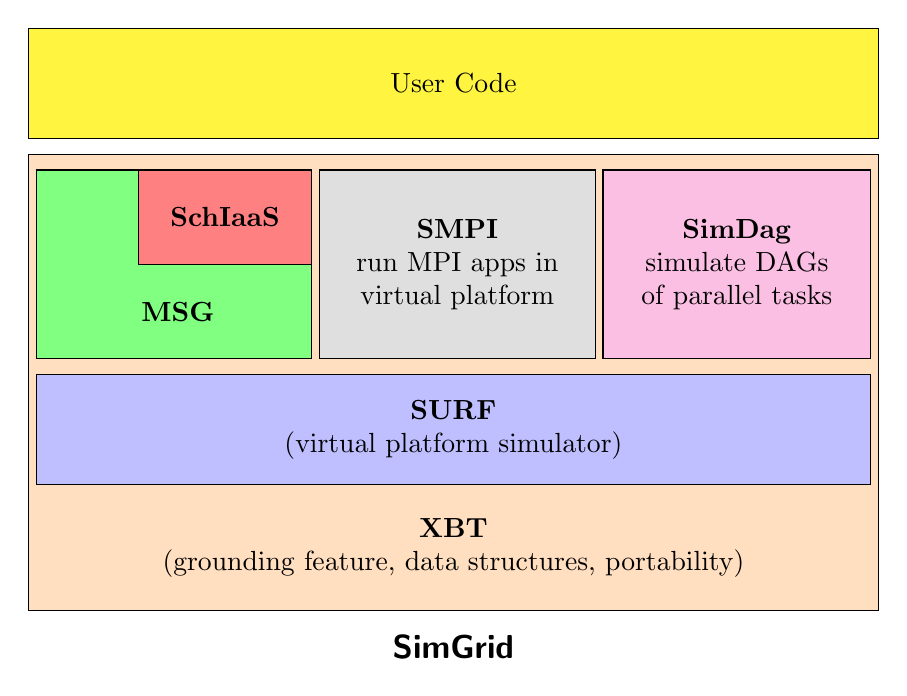
\begin{tikzpicture}[x=1cm,
y=1cm,
every node/.style={
rectangle,
align = center,
anchor=south west,
outer sep=1mm,
},
box/.style={
draw,
}]

%Simgrid box
\node[box,minimum height=5.8cm,minimum width=10.8cm,fill=orange!25,label={south:\large{}\textsf{\textbf{SimGrid}}}]at(0,0){};
%\node[box,minimum height=5.8cm,minimum width=1.4cm,fill=cyan!50]at(11,0){\rotatebox{270}{\textbf{Tracing}}};
\node[minimum height=1.4cm,minimum width=10.6cm]at(0.1,0.1){\textbf{XBT}\\(grounding feature, data structures, portability)};
\node[box,minimum height=1.4cm,minimum width=10.6cm,fill=blue!25]at(0.1,1.6){\textbf{SURF}\\(virtual platform simulator)};
\node[box,minimum height=2.4cm,minimum width=3.5cm,fill=green!50]at(0.1,3.2){};
\node[box,minimum height=2.4cm,minimum width=3.5cm,fill=gray!25]at(3.7,3.2){\textbf{SMPI}\\run MPI apps in\\ virtual platform};
\node[box,minimum height=2.4cm,minimum width=3.4cm,fill=magenta!25]at(7.3,3.2){\textbf{SimDag}\\simulate DAGs\\ of parallel tasks};

\node[box,minimum height=1.2cm,minimum width=2.2cm,fill=red!50]at(1.4,4.4){\textbf{SchIaaS}};
\node[minimum height=1.2cm,anchor=south]at(2,3.2){\textbf{MSG}};

\node[box,minimum height=1.4cm,minimum width=10.8cm,fill=yellow!75]at(0,6){User Code};
\end{tikzpicture}
}
\caption{The  layered  architecture of  SimGrid,  with  the additionnal  SchIaaS
  interface}
\label{fg:sg-archi}
\end{figure}


In this general  picture, SCHIaaS is a new interface  upon MSG. SCHIaaS entities
use MSG  to communicate with  the core functions  of SimGrid, which  handles the
operating  system  level  objects,   such  as  network  communications,  running
processes, and  virtual machines. SCHIaaS entities  are mainly \emph{instances}.
We use the term \emph{instance}, as popularized by AWS, to designate the virtual
machine when  seen from  the client  side. Accordingly,  the SchIaaS  API offers
cloud level functionalities,  that is the operations usually  provided by public
cloud  providers: run,  terminate, suspend,  resume and  describe instances  and
operations regarding cloud  storage. For sake of modeling a  cloud, SchIaaS also
allows the  user to  describe the  available resources,  the image  and instance
types management, the  VM placement policy on the  clusters and operating-system
levels parameters such as boot and other VM life-cycle processes.  By constrast,
SimGrid implements hypervisor level functionalities  such as starting or stoping
a \ac{vm}.


\subsection{SCHIaaS's design}

Developped  in Java,  SCHIaaS  has been  designed as  a  modular and  extensible
framework, allowing modelers to plugin their  own code in all the key components
which model  the cloud  or application behavior  under study.   Figure \ref{fg:}
zooms in  the SCHIaaS box  of Figure~\ref{fg:sg-archi}. It shows  the components
making up SCHIaaS (in  the red box). The boxes with  dashed frames indicate that
these can be replaced with user-provided code.
%
\begin{figure}[hbt]
\centering
\resizebox{.7\textwidth}{!}{%
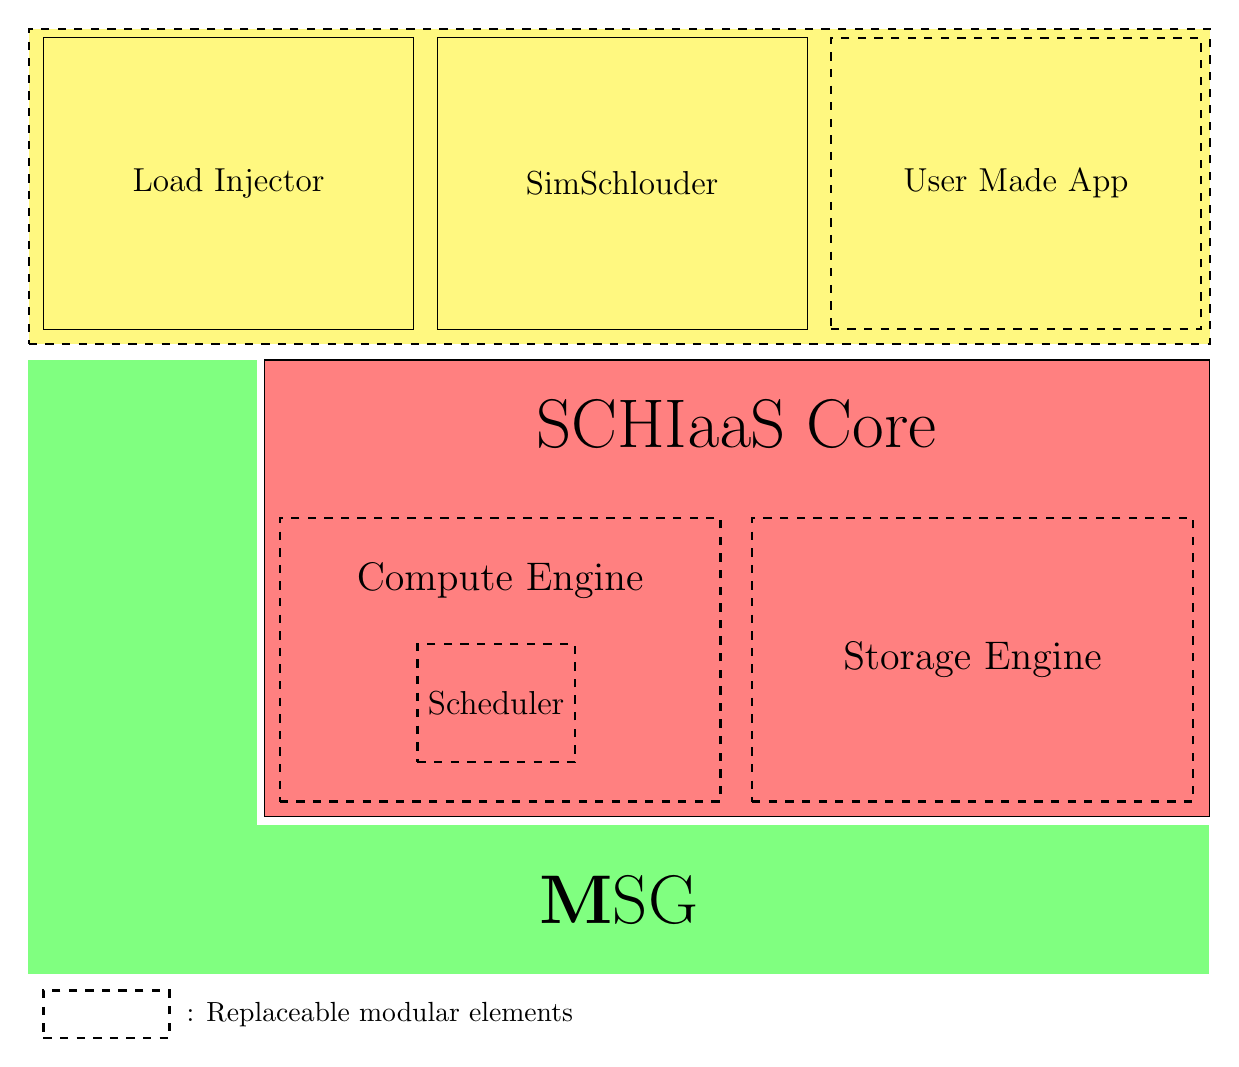
\begin{tikzpicture}[
every node/.style={anchor = south west,},
legend/.style={anchor=north west,dashed,thick,outer sep=2mm,minimum height=0.6cm},
plug/.style={dashed,thick,text=black},
sub/.style={draw,outer sep=2mm},
tag/.style={anchor=center,align=center},
engine/.style={minimum height=3.6cm,minimum width=5.6cm,plug},
sched/.style={minimum height=1.5cm,minimum width=2cm,plug},
app/.style={minimum height=3.7cm,,minimum width=4.7cm},
]
%\draw[help lines](0,0)grid(15,15);
\node[fill=green!50,minimum height=6.9cm,minimum width=2.9cm]at(0,0.9){};
\node[fill=green!50,minimum height=1.9cm,minimum width=15cm]at(0,0){\Huge \textbf MSG};

\node[draw,fill=red!50,minimum height=5.8cm,minimum width=12cm]at(3,2){};
\node[tag]at(9,7){\Huge SCHIaaS Core};
\node[sub,engine]at(3,2){};
\node[tag]at(6,5){\Large{}Compute Engine};
\node[sub,sched]at(4.75,2.5){\large{}Scheduler};
\node[sub,engine]at(9,2){};
\node[tag]at(12,4){\Large Storage Engine};

\node[plug,fill=yellow!50,draw,minimum height=4cm,minimum width=15cm]at(0,8){};
\node[sub,app]at(0,8){\large{}Load Injector};
\node[sub,app]at(5,8){\large{}SimSchlouder};
\node[sub,app,plug]at(10,8){\large{}User Made App};

%Legend
\node[legend,draw,minimum width=1.6cm]at(0,0){};
\node[legend]at(1.7,0){: Replaceable modular elements};

\end{tikzpicture}
}
\caption{Zoom on the SCHIaaS framework}
\label{fg:}
\end{figure}
%
\paragraph{SCHIaaS Core} contains all the management code necessary to set up the data
  structures corresponding of the cloud described in the configuration file, and
  to reflect the effects on the  data structures of all the operations triggered
  though the Compute and Storage engines.

\paragraph{The  Compute Engine} provides  an interface for  the management of  VMs. It
  expects  an  implementation of  the  way  the  cloud controller  controls  the
  instances,  through the  definition of  start, shutdown,  suspend, resume  and
  reboot commands. It also expects  an implementation of the scheduling policies
  used to map instances onto physical machines.

\paragraph{The Storage  Engine}  offers  an interface  for  the  management of  block
  storage, through the definition of put, get, delete, and list operations.\\

\noindent %
In order to model a system SimGrid requires two configuration files: 
\begin{itemize}
\item a \emph{plaform}  file describing the available  hardware, including hosts
  capabilities (e.g number of cores, CPU power) and a description of the network
  (e.g interconnection topology and network link performances),
\item a \emph{deployment} file which maps the applicative processes to some of
  the hosts described in the platform.
\end{itemize}

SCHIaaS adds  to these  a third  configuration file to  describe one  or several
clouds.   An example  configuration  is shown  in Figure~\ref{fg:cloud.xml},  in
which the  default implementations that  come with the SCHIaaS  distribution are
used.  The \emph{storage} and \emph{compute}  sections correspond to the storage
and compute  engines listed  above.  Each  of these component  are handled  by a
\emph{controller}   bound  to   some  host   in  the   SimGrid  platform   file.
Implementations of  the controller's behavior,  that is the storage  and compute
engine  instanciations, appear  line  2  and 6.   For  the  compute engine,  the
specific  scheduling  policy  which  computes  how VMs  are  mapped  to  PMs  is
implemented in  the attached scheduler module  line 10.  Note that  each request
that the controller sends to the cluster nodes, be it a simple command or a data
transfer, generates network communications that are simulated by SimGrid.

\begin{figure}[hbt] 
 \lstset{language=xml,label= ,caption= ,numbers=left}
\begin{lstlisting}
<cloud  id="myCloud">
   <storage id="myStorage" engine="org.simgrid.schiaas.engine.storage.rise.Rise">
      <config controller="controller"/>
   </storage>

   <compute engine="org.simgrid.schiaas.engine.compute.rice.Rice"> 		
      <config controller="controller" image_storage="myStorage"
              image_caching="PRE" inter_boot_delay="10"/>
  
      <scheduler name="org.simgrid.schiaas.engine.compute.scheduler.SimpleScheduler"
                 type="consolidator"
                 controller="controller"
                 delay="1"/>
  
      <instance_type id="small" core="1" memory="1000" disk="1690" />				
      <instance_type id="medium" core="2" memory="1000" disk="1690"/>
      <instance_type id="large" core="4" memory="1000" disk="1690"/>
  
      <image id="myImage" size="1073741824"/>
      <cluster id="my_cluster" prefix="node-" suffix=".me" radical="1-"/>  
    </compute>
</cloud>
\end{lstlisting}
\caption{An example \texttt{cloud.xml} file describing the environment of a
  given cloud, including the custom java classes used to implement the
  cloud controller behavior.}
\label{fg:cloud.xml}
\end{figure}


%------ This is the actual system we model through simulation -------------------
\section{Case Study}
\label{sc:context}

In the first part of this article

As  mentioned   in  introduction,  complex  workloads   require  scheduling  and
provisionning tools, and we present in  this section the cloud management system
together with the actual hardware setup we run to handle these experiments.

\subsection{Schlouder}

Every  experiment log  in  the archive  was generated  by  running a  scientific
workflow  through a  client-side  cloud resource  broker named  \emph{Schlouder}
\cite{Michon17}. \emph{Schlouder} automates the provisioning of resources needed
to execute a workflow, the scheduling of tasks to the provisioned resources and,
monitors the proper execution of tasks.
%
\begin{figure}
	\centering
	\usetikzlibrary{fit,arrows}
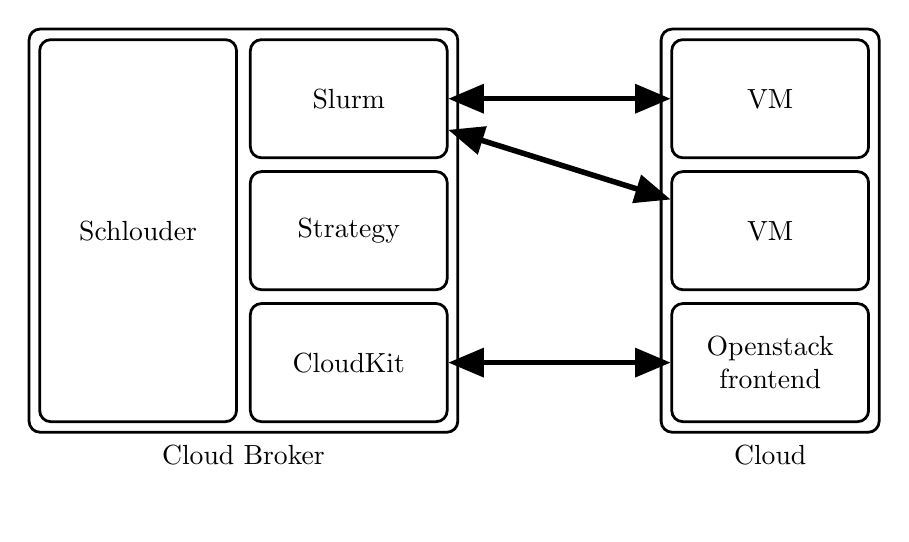
\begin{tikzpicture}[node distance=5pt,x=25mm+5pt,y=15mm+5pt,
every node/.style={anchor=center,
line width=1pt,
minimum width = 25mm,
minimum height =15mm,
rounded corners,
label distance=-5mm,
draw 
},
high/.style={%
minimum height =45mm+10pt,
},
large/.style={%
minimum width=50mm+5pt
}]
\node[high]at(0,0)(app){Schlouder};
\node[]at(1,-1)(ck){CloudKit};
\node[]at(1,0)(strat){Strategy};
\node[]at(1,1)(slm){Slurm};
\node[align=center]at(3,-1)(cc){Openstack\\frontend};
\node[]at(3,0)(vm1){VM};
\node[]at(3,1)(vm2){VM};
\node[draw,fit=(app)(ck)(slm),label={below:Cloud Broker}]{};
\node[draw,fit=(vm2)(cc)(vm1),label={below:Cloud}]{};
\draw [{triangle 45}-{triangle 45},line width=2pt] (ck)--(cc);
\draw [{triangle 45}-{triangle 45},line width=2pt] (vm2)--(slm);
\draw [{triangle 45}-{triangle 45},line width=2pt] (vm1)--(slm);
%\draw [{triangle 45}-{triangle 45},shorten <=10pt,shorten >=10pt] (1,0)--(1,1);
%\draw [{triangle 45}-{triangle 45},shorten <=10pt,shorten >=10pt] (1,0)--(1,-1);
\end{tikzpicture}

	\caption{The Schlouder cloud broker and its components relating to an
	Openstack cloud.}
\end{figure}
%
Provisioning is  done through  a cloud  kit interface  that allows  Schlouder to
communicate with  different clouds  in order  to start  and stops  the necessary
\acp{vm} to  execute the  workload.  To  account for  the pricing  of commercial
IaaS, Schlouder views  provisioning in fixed increments of time,  referred to as
\ac{btu},  machines  idle  when arriving  at  the  end  of  their time  will  be
automatically shut off.
%
Tasks execution  is monitored using  SLURM~\cite{YooJG03} which connects  to the
available \acp{vm}, send the jobs, and monitors their executions.

A strategy controls provisioning and scheduling decisions, it determines when
\ac{vm} provisioned and to which \ac{vm} each task is assigned. Schlouder
provides a few basic strategies and new ones can be added trivially. Strategies
can affect the workload's \emph{makespan}, the \acp{vm} usage rate, and the
number of opened \acp{btu} (i.e.\ the price of the experiment on a commercial
cloud). The experiments in our archive mainly use two strategies, \ac{asap} and
\ac{afap}

\begin{description}
	\item[\ac{asap}] will attempt to execute tasks as early as possible by
		booting a new \ac{vm} unless a \ac{vm} is already idle or one is
		predicted to become idle faster than a \ac{vm} can boot.
	\item[\ac{afap}] will favor scheduling tasks on already opened \ac{vm}
		unless doing is predicted extend the \ac{vm} runtime by an
		additional \ac{btu}, in which case it will boot a new \ac{vm}.
\end{description}

Predicted  tasks runtimes,  as well  as tasks  dependencies, are  user-provided.
Scheduling is  done dynamically, as  soon as tasks  are submitted and  all their
dependencies have been completed. Once assigned to a designated \ac{vm} jobs are
not rescheduled. However, if a \ac{vm}  fails to boot Schlouder will provision a
new one to replace it.

%---------------------------- H A R D W A R E-----------------------------------
\subsection{Hardware Setup}

Evaluation  of simulation  is done  by comparing  simulation logs,  against logs
generated by running  actual scientific workflows on  multiple platforms. During
this  study  we   gathered  traces  for  274  experimental   executions  on  two
significantly different environments that are described hereafter.


\paragraph{Private Cloud}

Our private cloud is based on two local nodes sporting dual $2.64GHz$ Intel Xeon
processors (X5650),  for a  total of  96 cores. Nodes  operated on  Ubuntu 12.04
distributions and virtualisation  is achieved using KVM.  Openstack 2012.1.3 was
used as a  cloud interface. This cloud was build  on perfectly homogeneous nodes
and  devoid  of other  users.  For  data storage  these  experiments  rely on  a
\ac{nfs}. Special  attention was taken  to not  overbook \acp{vm} by  caping the
number of  single core \acp{vm}  to 25. Due to  the experimental nature  of this
cloud configurations  have change  overtime. Table  \ref{tab:platforms} regroups
configurations  of  all cloud  versions.  We  will  referrer  to this  cloud  as
\texttt{openstack-icps.}\emph{version}.


\paragraph{Public Cloud}

BonFire~\cite{Kavoussanakis2013} is  a public  multi-cloud distributed  all over
Europe. Our experiments  were run over three sites of  BonFire: de-hlrs based in
Stuttgart, uk-epcc  in Edinburgh,  and fr-inria in  Rennes. BonFIRE  clouds were
accessed  through an  OCCI based  API and  the clouds  were controlled  throught
software derived from OpenNebula 3.6.  Each site provided different hardware%
\footnote{Comprehensive            information           available            at
  \texttt{http://www.bonfire-project.eu/infrastructure/testbeds}}.%
Resource quotas  limited most experiment  20 \acp{vm},  not far from  the limits
generally imposed on  public clouds. Centralized storage was  provided through a
\ac{nfs} based on  the be-ibbt site in Ghent.  Due  to network acces restriction
the Schlouder server was  brought in the BonFIRE WAN through a  VPN.  Due to the
experimental nature  of this  cloud configurations  have change  overtime. Table
\ref{tab:platforms}  regroups  configurations of  all  cloud  versions. In  this
article we  refer to experiment  run on  the BonFire clouds  by the name  of the
cloud site followed by the version number.

\begin{table}
	\begin{tabular}{|l|c|c|c|c|c|c|}
		\hline
		Cloud&\#cores&Hypervisor&Network&version&\#VM&Storage\\ \hline
		\multirow{2}{*}{openstack-icps}&\multirow{2}{*}{48}&
                \multirow{2}{*}{KVM}&100mb&1-3&25&NFS\\\cline{4-7}
		&&&1Gb&4-5&10&NFS\\\hline
		de-hlrs&344&Xen 3.1.2&n/a&v1-3&20&NFS\\\hline
		fr-inria&96&Xen 3.2&n/a&v1-3&20&NFS\\\hline
		uk-epcc&176&Xen 3.0.3&n/a&v1-2&20&NFS\\\hline

	\end{tabular}
	\caption{Characteristics of our cloud testbeds, version numbers also
	account for changes in measured boot times not presented in this table.}
	\label{tab:platforms}
\end{table}


\subsection{Use cases: Applications characteristics}
\label{sc:app}

Our study is  based on the experimentation with two  test-case applications that
cover a variety of application profiles  in terms of computation intensity, data
load, and task dependency.

\subsubsection{OMSSA}

The \ac{omssa}~\cite{Geer2004}  comes from the  field of  biology, it is  used in
tandem mass  spectrometry analysis  (also known as  MS/MS analysis)  to identify
peptides   from   the   mass   and    fragment   ions   obtained   by   a   mass
spectrometer. \ac{omssa} matches measurements from the mass spectrometer, called
spectra, to a protein database.

The \ac{omssa}  workload features fully  independent tasks, making  it \ac{bot},
since every spectra  within a set can be submitted  independently to \ac{omssa}.
With a  \emph{communication-to-computation} ratio comprised between  20\% and \%
\ac{omssa} is considered an CPU-intensive workload.

This application was run with 4 different workload covering 2 different
mass~spectrometer resolutions of two different protein solutions, denoted
\emph{brs},\emph{hrs},\emph{brt} and \emph{hrt}.

\subsubsection{Montage}

The Montage  Astronomical Image Mosaic Engine~\cite{montage2009}  is designed to
gather  astronomical images  into  a  mosaic.  This  application  is a  workflow
designed to reproject, normalize, and collate source images into a single output
image. The montage workflow  is presented figure~\ref{fig:montagewf}. Working on
images   Montage   is   an   extremely    data   intensive   workflow   with   a
\emph{communication-to-computation} ratio superior to 90\%. This application was
run on  images of the \emph{Pleiade}  star cluster at 3  different output sizes,
1X1, 2X2 and 3X3.

\begin{figure}[ht]
	\usetikzlibrary{fit,arrows}
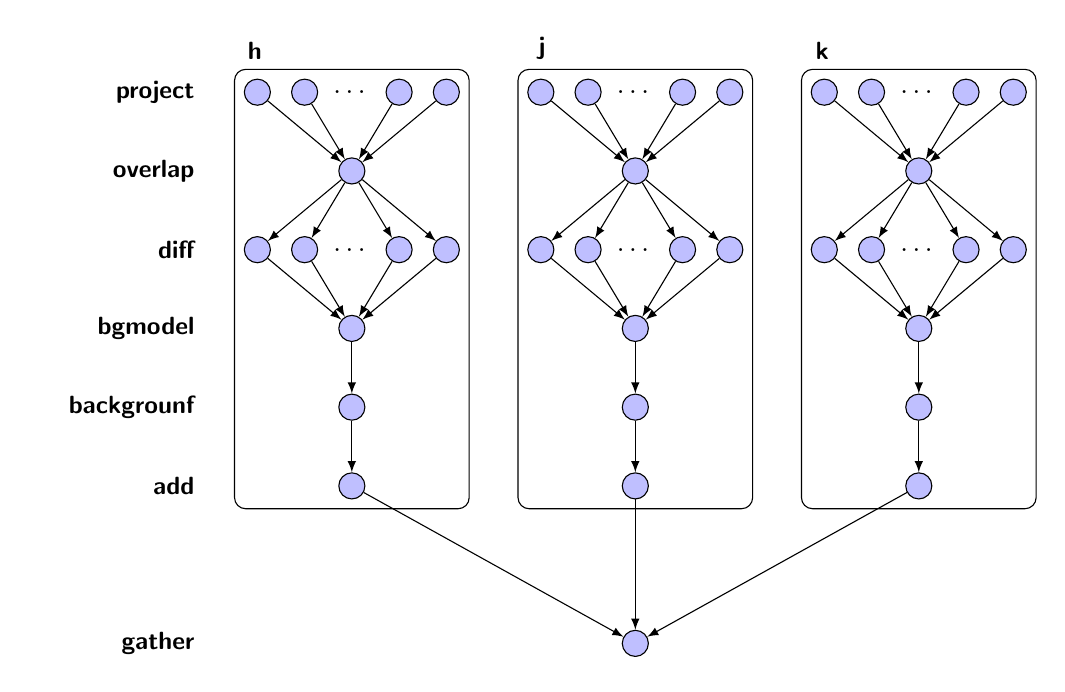
\begin{tikzpicture}[x=6mm,y=-10mm,
task/.style={%
 fill=blue!25,
draw,circle
},
level/.style={%
  font={\sffamily\bfseries\color{black} \fontsize{9pt}{12}\selectfont},
  align=right,
  text width=20mm
},
dot/.style={%
circle
}
]
%levels
\node[level] at (0,0)(Lproj){project};
\node[level] at (0,1)(Loverlap){overlap};
\node[level] at (0,2)(Ldiff){diff};
\node[level] at (0,3)(Lbgm){bgmodel};
\node[level] at (0,4)(Lbg){backgrounf};
\node[level] at (0,5)(Ladd){add};
\node[level] at(0,7)(Lgather){gather};
%%Gather node
\node[task,shift={(9,0)}]at(2,7)(gather){};
%%Loop HJK
\foreach \n [count=\i from 0] in {h,j,k}
{%
\begin{scope}[shift={(3+6*\i,0)}]
% 1 node per group
\node[task]at(2,1)(\i_overlap){};
\node[task]at(2,3)(\i_bgm){};
\node[task]at(2,4)(\i_bg){};
\node[task]at(2,5)(\i_add){};
%% 4 node per group
\foreach \y in {0,1,3,4}
{%
\node[task]at(\y,0)(\i_p_\y){};
\node[task]at(\y,2)(\i_d_\y){};
\draw[-{latex}](\i_p_\y)--(\i_overlap);
\draw[-{latex}](\i_overlap)--(\i_d_\y);
\draw[-{latex}](\i_d_\y)--(\i_bgm);
}
%%4 groups elipsis
\foreach \y in {0,2}
{%
\node[dot]at(2,\y){\ldots};
}
%%single deps
\draw[-{latex}](\i_bgm)--(\i_bg);
\draw[-{latex}](\i_bg)--(\i_add);
%%HJK boxes
\node[rounded corners,draw,fit=(\i_add)(\i_p_0)(\i_p_4),label={[font={\sffamily\bfseries\color{black}\fontsize{9pt}{12}\selectfont}]110:\n}]{};
\end{scope}
%% Gather deps
\draw[-{latex}](\i_add)--(gather);
}
\end{tikzpicture}
	\caption{Illustration of the Montage workflow. Each node represents a
	tasks and each arc represents a data dependency between two tasks. Every
	task on a specific row run the Montage command indicated on the left
	hand side of the graph.}
	\label{fig:montagewf}
\end{figure}

%-------------------------- S I M U L A T E D --------------------------------
\section{Simulation}
\label{sc:simulation}

\subsection{Using SCHIaaS to simulate Schlouder}


\center{\textbf{Ici, raconter comment SimSchlouder a été écrit}.



%-------------------------- E V A L U A T I O N -------------------------------  
\subsection{Evaluation}

The evaluation of the simulation accuracy of such a system is both a complex and
tedious task.  It  is complex because the simple comparison  of the observed and
predicted walltimes is not sufficient for  the experimenter to be aware of which
parts of the execution are correctly or wrongly simulated and how much each part
impacts the whole simulation. During the process of comparison, the experimenter
often  has  to add  extra  watch  points into  the  application  and re-run  the
experiment to  eventually obtain the  relevant measurements.  This is  a tedious
back  and forward  process  which  generally increases  the  number of  observed
parameters and makes execution log traces heterogeneous over time.

\subsubsection{Lab}

% TODO @Julien
éléments concrets pour le lab (c.f Renpar).

Le  lab est  un ensemble  de  scripts permettant  d'automatiser l'exécution  des
simulations, la  collecte des  observations, ainsi que  leur analyse.  Il permet
donc d'exécuter  de bout-en-bout  l'étude par simulation,  de la  définition des
différentes simulations, à la production des graphiques.

Au delà de l'aspect pratique et du gain de temps de mise en œuvre de l'étude, le
lab a pour vocation de ``standardiser'' l'étude. Cette standardisation assure sa
reproductibilité, ainsi qu'une  comparaison équitable entre solutions  à un même
problème.

Mais  le   lab  permet   également  une   approche  systématique   permettant  à
l'expérimentateur de  ne pas rater  de phénomène. En  effet, il est  fréquent de
faire un  grand lot  de simulations,  puis d'observer  plus finement  celles qui
présentent des  particularités. Ce  faisant, l'expérimentateur exclu  les autres
simulation  de  ces   observations  plus  précises,  à  moins   de  les  refaire
entièrement. En rendant plus pratique la définition des observations directement
au niveau  du \textit{workflow} de simulations,  le lab assure que  tous les cas
seront observés de  la même manière, ce  qui évite de rater un  phénomène, ou de
différencier le traitement des simulations au risque d'arriver à des conclusions
abusives.




\subsubsection{Procedural Analysis}

Démarche expérimentale de validation du simulateur.

Process de simulation : choisir l'application, définir les métriques, executer 

Voici la procédure expérimentale que nous avons employé:
Sur ce type d'application nous avons besoin des informations 

\begin{enumerate}
 \item Real executions (xp) to test Schlouder and provisioning/scheduling 
strategies.
  Schlouder/SimSchlouder input:
  \begin{itemize}
   \item Nodes: boottime prediction, amount of instances limit, standard power
   \item Tasks: walltime prediction
  \end{itemize}
 
 \item Normalization of xp traces (4 versions of schlouder, missing data)
 \item Extraction of information about each xp:
  \begin{itemize}
   \item Instance: provisioning date, start date, end date, boottimes, instance 
type
   \item Tasks: submission date, scheduling date, start date, end date, 
	  walltime, input time and size, runtime, output time and size, 
management time
  \end{itemize}
 \item Simulation of each xp, injecting different information from real xps
 \item Comparison of Schlouder and SimSchlouder outputs (python)
 \item Statistical analysis of all traces (R) : distribution de l'erreur
            
 \item Close analysis of each outlier to understand the differences. 
\end{enumerate}





\subsubsection{life-cycles and observed times}

\begin{itemize}
 \item Execution: $e \in E$
 \item Node of execution $e$: $n \in N_e$
 \item Task of execution $e$: $t \in T_e$
 \item Task handled by node $n$: $t \in T_n$
 \item The node running the task $t$ is denoted $n_t \in N$
 \item $v^R$ denotes the value $v$ in the rality
 \item $v^S$ denotes the value $v$ in the simulation
 \item 
\end{itemize}

During the execution, the node are in the following states:

\begin{figure}
\resizebox{\textwidth}{!}{%
%\minibox[c]{
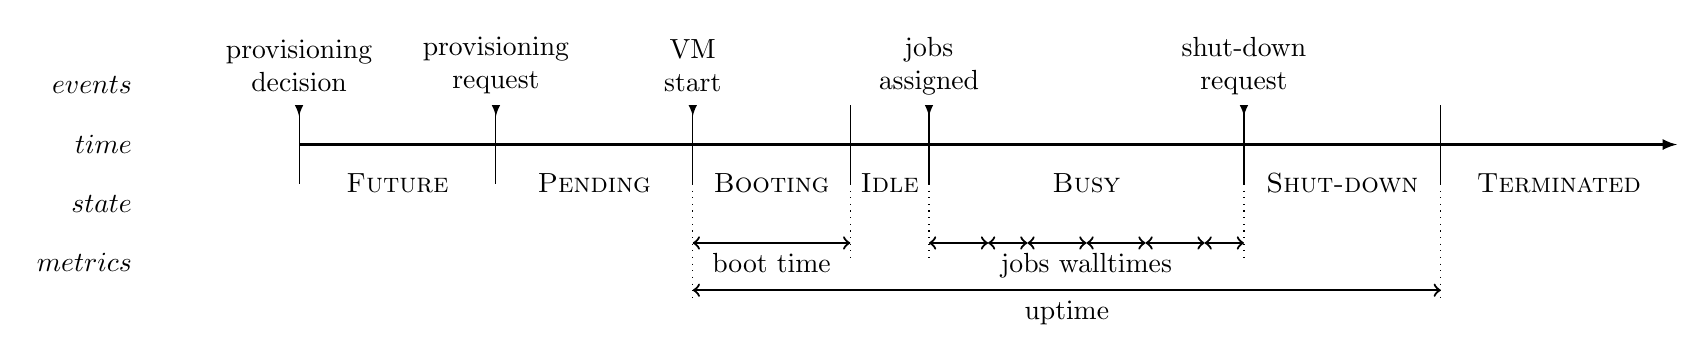
\begin{tikzpicture}[
legend/.style={anchor=east,align=right},
event/.style={align=center,outer sep=1},
status/.style={anchor=north,align=center,font=\sc},
metric/.style={<->,thick},
]
%legend
\node[legend]at(-1,0.75){$events$};
\node[legend]at(-1,0){$time$};
\node[legend]at(-1,-0.75){$state$};
\node[legend]at(-1,-1.5){$metrics$};
%axis
\draw[-{latex},thick](1,0)--(18.5,0);
%marker - event - following status
%provisioning decision
\draw[{latex reversed}-](1,0.5)->(1,-0.5);
\node[event]at(1,1){provisioning\\decision};
\node[status]at(2.25,-0.25){Future};
%provisioning
\draw[{latex reversed}-](3.5,0.5)->(3.5,-0.5);
\node[event]at(3.5,1){provisioning\\request};
\node[status]at(4.75,-0.25){Pending};
%booting
\draw[{latex reversed}-](6,0.5)--(6,-0.5);
\draw[dotted](6,-0.5)--(6,-2);
\node[event]at(6,1){VM\\start};
\node[status]at(7,-0.25){Booting};
%idle
\draw (8,0.5)--(8,-0.5);
\draw[dotted](8,-0.5)--(8,-1.5);
%\node[event]at(8.5,1){};
\node[status]at(8.5,-0.25){Idle};
%Assign jobs
\draw[{latex reversed}-](9,0.5)--(9,-0.5);
\draw[dotted](9,-0.5)--(9,-1.5);
\node[event]at(9,1){jobs\\assigned};
\node[status]at(11,-0.25){Busy};
%Shutdown
\draw[{latex reversed}-](13,0.5)--(13,-0.5);
\draw[dotted](13,-0.5)--(13,-1.5);
\node[event]at(13,1){shut-down\\request};
\node[status]at(14.25,-0.25){Shut-down};
%terminated
\draw(15.5,0.5)--(15.5,-0.5);
\draw[dotted](15.5,-0.5)--(15.5,-2);
\node[status]at(17,-0.25){Terminated};

%Metrics
\draw[metric](6,-1.85)--(15.5,-1.85) node[midway,below]{uptime};
\draw[metric](6,-1.25)--(8,-1.25) node[midway,below]{boot time};
\draw[metric](9,-1.25)--(9.75,-1.25);
\draw[metric](9.75,-1.25)--(10.25,-1.25);
\draw[metric](10.25,-1.25)--(11,-1.25) node[below]{jobs walltimes};
\draw[metric](11,-1.25)--(11.75,-1.25);
\draw[metric](11.75,-1.25)--(12.5,-1.25);
\draw[metric](12.5,-1.25)--(13,-1.25);

\end{tikzpicture}
%}
}
\caption{Nodes' states}
\end{figure}

\begin{figure}
\resizebox{\textwidth}{!}{%
%\minibox[c]{
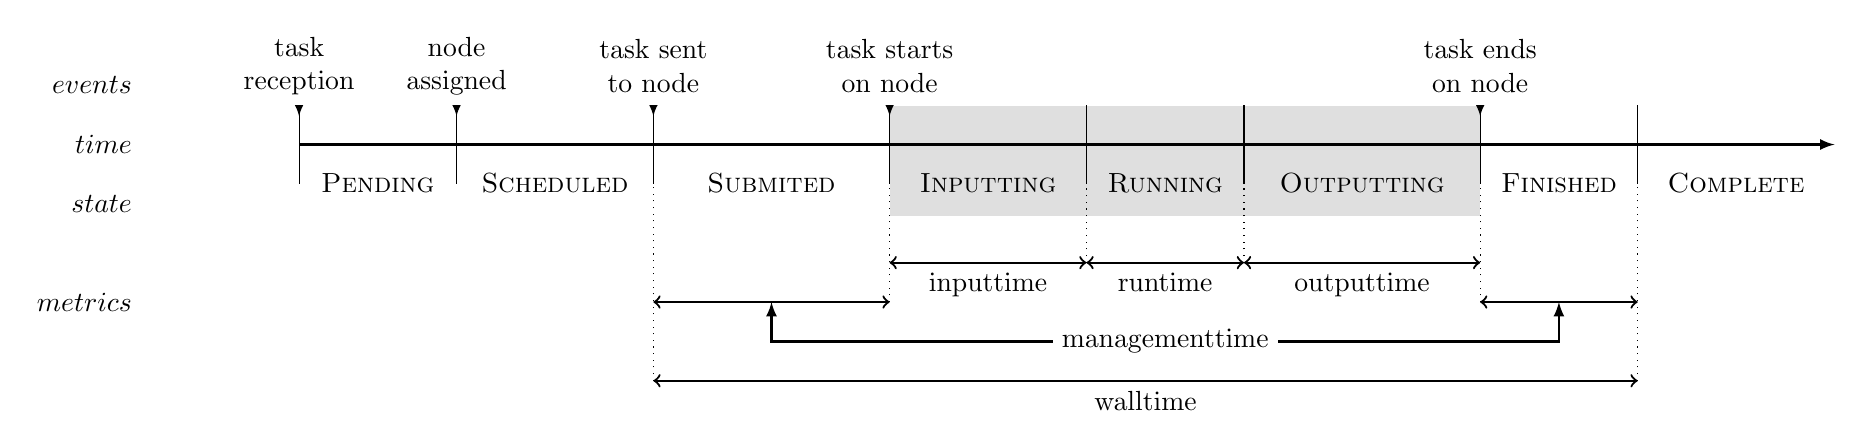
\begin{tikzpicture}[
legend/.style={anchor=east,align=right},
event/.style={align=center,outer sep=1},
status/.style={anchor=north,align=center,font=\sc},
metric/.style={<->,thick},
]
%legend
\node[legend]at(-1,0.75){$events$};
\node[legend]at(-1,0){$time$};
\node[legend]at(-1,-0.75){$state$};
\node[legend]at(-1,-2){$metrics$};

\node[rectangle,fill=gray!25,anchor=north west,minimum height=40,minimum width=213]at(8.5,0.5){};
%axis
\draw[-{latex},thick](1,0)--(20.5,0);
%marker - event - following status

%submition
\draw[{latex reversed}-](1,0.5)->(1,-0.5);
\node[event]at(1,1){task\\reception};
\node[status]at(2,-0.25){Pending};
%scheduling
\draw[{latex reversed}-](3,0.5)--(3,-0.5);
\node[event]at(3,1){node\\assigned};
\node[status]at(4.25,-0.25){Scheduled};
%sending
\draw[{latex reversed}-](5.5,0.5)--(5.5,-0.5);
\node[event]at(5.5,1){task sent\\to node};
\node[status]at(7,-0.25){Submited};

%download
\draw[{latex reversed}-](8.5,0.5)--(8.5,-0.5);
\node[event]at(8.5,1){task starts\\on node};
\node[status]at(9.75,-0.25){Inputting};
%exec
\draw(11,0.5)--(11,-0.5);
\node[status]at(12,-0.25){Running};
%output
\draw(13,0.5)--(13,-0.5);
\node[status]at(14.5,-0.25){Outputting};
%finish
\draw[{latex reversed}-](16,0.5)--(16,-0.5);
\node[event]at(16,1){task ends\\on node};
\node[status]at(17,-0.25){Finished};
%complete
\draw(18,0.5)--(18,-0.5);
\node[event]at(18,1){};
\node[status]at(19.25,-0.25){Complete};

%metrics
\draw[dotted](5.5,-3)--(5.5,-0.5);
\draw[dotted](18,-3)--(18,-0.5);
\draw[metric](5.5,-3)--(18,-3)node[midway,below]{walltime};

\draw[dotted](8.5,-2)--(8.5,-0.5);
\draw[dotted](11,-1.5)--(11,-0.5);
\draw[dotted](13,-1.5)--(13,-0.5);
\draw[dotted](16,-2)--(16,-0.5);
\draw[metric](8.5,-1.5)--(11,-1.5)node[midway,below]{inputtime};
\draw[metric](11,-1.5)--(13,-1.5)node[midway,below]{runtime};
\draw[metric](13,-1.5)--(16,-1.5)node[midway,below]{outputtime};

\draw[metric](5.5,-2)--(8.5,-2);
\draw[metric](16,-2)--(18,-2);
\draw[{latex}-{latex},thick](7,-2)--(7,-2.5)--(17,-2.5)node[midway,fill=white]{managementtime}--(17,-2);

\end{tikzpicture}

%}
}
\caption{Tasks' states}
\end{figure}

\begin{comment}
\begin{enumerate}
 \item Future: Once the decision to start the node is made;
 \item Pending: Once the node is requested to the cloud-kit;
 \item Booting: Once the cloud-kit aknowledge the satisfaction of the request;
 \item Idle: Once the node is ready to run tasks;
 \item Busy: Once the node is running one task;
 \item ShuttingDown: Once the termination of the node is aked to the cloud-kit;
 \item Terminated: Once the node is terminated.
\end{enumerate}
\end{comment}


The observed times are:
\begin{itemize}
 \item $uptime(n) = terminated_n - booting_n$ 
 \item $boottime(n) = idle_n - booting_n$ 
\end{itemize}


During the execution, the task are in the following states, each corresponding to one date:
\begin{enumerate}
 \item Pending: Once they are subitted to the system;
 \item Scheduled: Once the system decided on which node the taks should be executed;
 \item Submitted: Once the task is sent to the worker node;
 \item Inputting: Once the task begin to download its data;
 \item Running: Once the task begin to computed;
 \item Outputting: Once the task begin to upload its result;
 \item Finished: Once the task is finished;
 \item Complete: Once the system aknowledge the completion of the task.;
\end{enumerate}

The observed times are:
\begin{itemize}
 \item $walltime(t) = complete_t - submitted_t$ 
 \item $inputtime(t) = running_t - inputting_t$
 \item $runtime(t) = outputting_t - running_t$
 \item $outputtime(t) = finished_t - outputting_t$
 \item $managementtime(t) = walltime_t - (inputtime_t+runtime_t+outputtime_t)$
 \item or $managementtime(t) = (inputting_t - submitted_t) + (complete_t - finished_t)$
\end{itemize}



\subsection{Discussion of Results}

\subsection{Definitions}
4 metrics $m \in M$ for each execution $e \in E$:
\begin{itemize}
 \item uptime: amount of rented resources, cost 
  $$uptime(e) = \sum_{n \in N_e} uptime_n$$
 \item makespan: duration of the xp from the submission of the first task to 
the end of the last task, user experience 
  $$makespan(e) = max_{t \in T_e} complete_t$$
 \item usage: runtime / uptime, efficiency of the provisioning 
  $$usage(e) = \frac{\sum_{t \in T_e} walltime_t}{\sum_{n \in N_e} uptime_n}$$
 \item schederror: number of tasks that are not assigned to the same node in 
the simulation compared to the reality, accuracy of the scheduling decisions
  $$schederror(e) = |t \forall t \in T / t_n^R \neq t_n^S|$$

\end{itemize}

Absolute errors are computed for each metric $m \in M$: 
$$m.ae(e) = \frac{| m^S(e) - m^R(e) |}{m^R(e)}$$

Results are shown as frequencies and statistics (stat = min, mean, median, max) 
of absolute errors occurrences. Frequencies are weighted so that the two applications
weigth the same, and the two platforms weigth alos the same 
(i.e. each couple application $\times$ platform represents 1/4th of the frequencies).

To compare absolute errors between set of simulations $S$ and $S'$
$S$ being the reference:
\begin{itemize}
 \item $\delta stat(m.ae(E)) = stat_{e \in E} ( m.ae^{S'}(e) ) - stat_{e \in E}( m.ae^S(e) )$
 \item $\Delta stat(m.ae(E)) = stat_{e \in E} ( m.ae^{S'}(e) - m.ae^S(e) )$
\end{itemize}




\subsection{Simulator accuracy}

Best simulation we can do.

Assess the raw simulator accuracy, injecting all real-life hazards that can be 
captured :
boottimes, walltimes and scheduling dates.

Scheduling dates allow to simulate some internal threaded mechanisms of 
Schlouder.
Schlouder uses two threads: the node manager and the task manager.
At settled intervals, the node manager interrupts the task manager to start and 
stop new nodes.
This changes the state of nodes, which influence provisioning and scheduling 
decisions.
However, simulating the exact moment of this interruption is utterly difficult, 
leading to differences between simulation and reality.


\begin{figure}
  \centering

  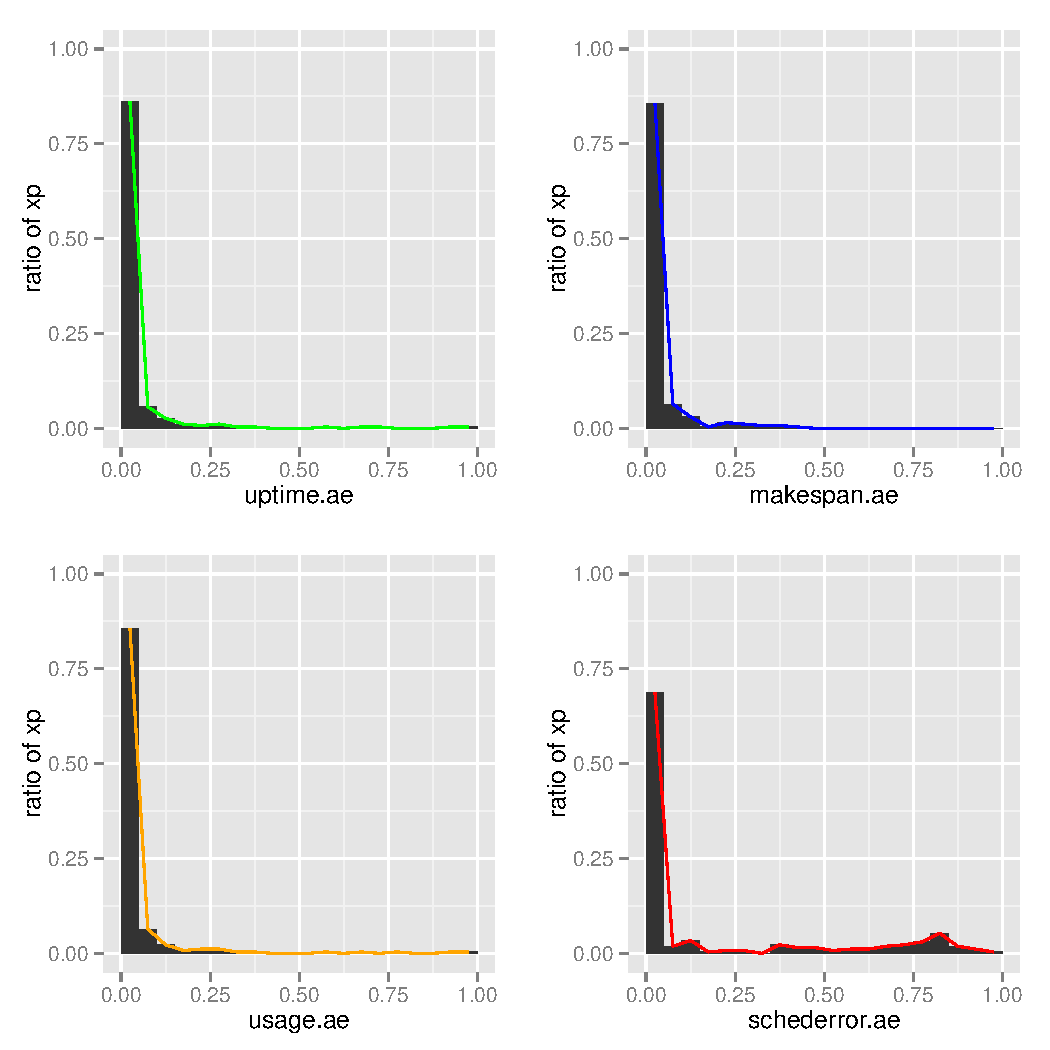
\includegraphics[width=\textwidth]{sim_best-4metrics.pdf}
  
  \input{\vrpath sim_best-4metrics-mmmm.latex}
  
\caption{Frequencies and statistics about absolute error of best simulations (274 xp)}
\end{figure} 

 


% see schiass/lab/setup/simschlouder/validation-results/best-4metrics.dat
\begin{itemize}
 \item uptime: 
      86\% show less than $0.05$ of absolute error, 
      92\% less than $0.10$, 
      2 simulations exceed $0.30$,
      ranging from $0.00$ to $0.50$, for a mean of $0.025$ and a median of $0.001$
 \item makespan: 
      76\% show less than $0.05$ of absolute error, 
      90\% less than $0.10$, 
      0 simulations exceed $0.30$,
      ranging from $0.00$ to $0.62$, for a mean of $0.042$ and a median of $0.018$
 \item usage: 
      59\% show less than $0.05$ of absolute error, 
      91\% less than $0.10$, 
      2 simulations exceed $0.30$,
      ranging from $0.00$ to $0.60$, for a mean of $0.043$ and a median of $0.002$
 \item schederror: 
      70\% show less than $0.05$ of absolute error, 
      72\% less than $0.10$, 
      59 simulations exceed $0.30$,
      ranging from $0.00$ to $0.965$, for a mean of $0.155$ and a median of $0.000$
\end{itemize}

If global metrics are quite accurately assessed by the simulator, 
the scheduling decisions can be very different between simulation and reality. 
One part of the explanation is that scheduling decisions are interdependent: 
any error leads to several others.


\subsection{Simulator accuracy according to platforms and applications}


\begin{figure}
  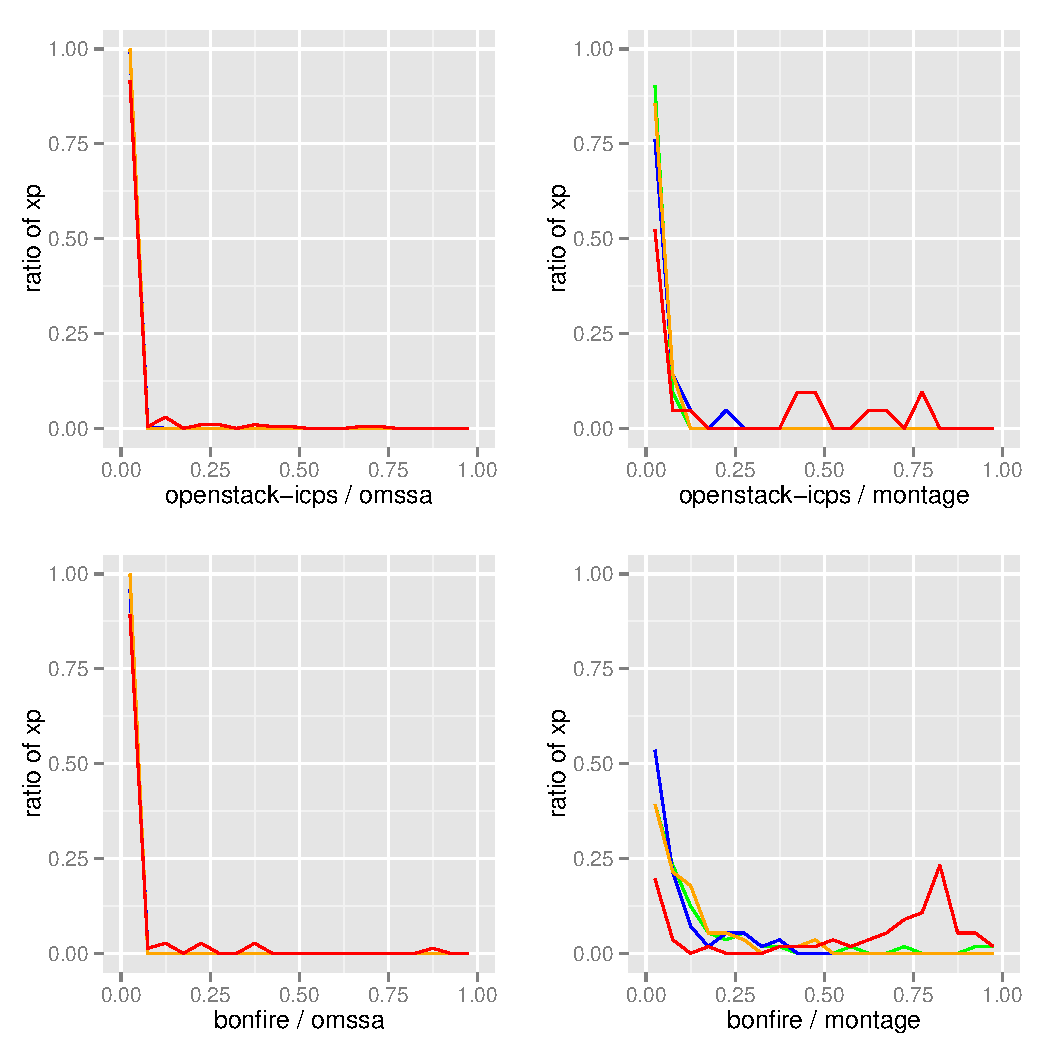
\includegraphics[width=\textwidth]{sim_best-4metrics-platform-app.pdf}
\caption{Absolute error frequencies of best simulations according to platforms 
and applications}
\end{figure} 

\begin{itemize}
 \item openstack-icps / omssa (107 xp): 
 
      \input{\vrpath sim_best-openstack-icps-omssa-4metrics-mmmm.latex}
 
      All metrics are almost perfectly assessed (mean AR from $0.001$ to $0.002$)
      except scheduling error 
      (mean $0.04$ and max $0.75$, 13\% of xp show at least one error), 
      leading to small makespan and usage errors. 
      
      We looked at each single case of scheduling error and all those errors 
      comes from ambiguities in the scheduling algorithms.
      
      This is a first limitation of simulation:
      Whenever heuristics lead to several equivalent solutions, 
      the decision is made by the implementation and relies on data structures 
      (e.g. selection of the first encountered suitable solution) or clocks 
      (e.g. the solution differs from a second to the next, which depends 
      on threads activations and timers). While we made sure to use the same 
      structures and timers, some clocks-related events can not be captured nor 
      simulated: Processing the nodes and tasks queues for scheduling and 
      provisioning decisions take time. Consequently, if those decisions rely on
      clock, they change during the decision process in reality, as clocks advance 
      by itself, but not in simulation, as clocks advance only explicitly.
      
      Thus, the simulation is not mistaken, but only different from reality.
      Actually, the decisions made by the simulator are exactly those that one 
      can expect, while the decisions made by the real scheduler are sometimes
      difficult to understand.

      
\begin{figure}  
  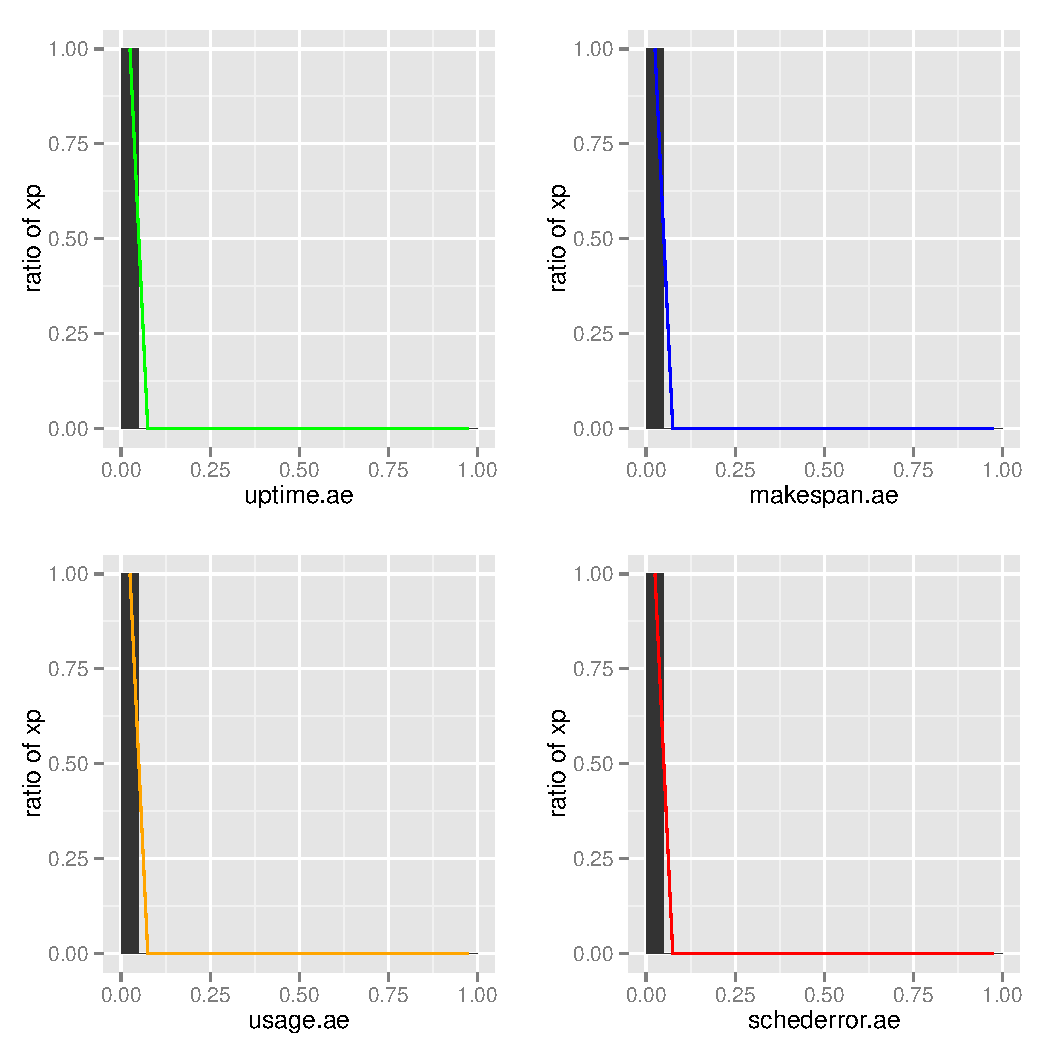
\includegraphics[width=\textwidth]{sim_best-openstack-icps-omssa-noschederror-4metrics.pdf}

  \input{\vrpath sim_best-openstack-icps-omssa-noschederror-4metrics-mmmm.latex}
      
  \input{\vrpath sim_best-openstack-icps-omssa-noschederror-4metrics-mmmm-cmp.latex}

\caption{Frequencies and statistics about absolute error of best simulations for openstack-icps / 
ommssa, without scheduling error cases (91 xps)}
\end{figure}       

      Filtering the xps showing clocks-related issues (16 xps), the results are perfect:
      all metrics present a mean ae of at most $0.001$.
      
      %Worst-case: v3.standard.hrt.asap.regular.openstack-icps.2
      The less accurate simulation shows a makespan absolute error of $0.010$. 
      Actually, the makespan of the simulation is $94s$, whereas it is $95s$ in reality.
      This small difference is due to one lag between two consecutive tasks 
      in the middle of the simulation. Such lags are not injected in our simulations.
      
      This shows that, providing that one can inject the right information, 
      the only limitation of our simulator are micro clock-related hazards.
      
      
 \item openstack-icps / montage (36 xps): 
 
      \input{\vrpath sim_best-openstack-icps-montage-4metrics-mmmm.latex}

      \input{\vrpath sim_best-openstack-icps-montage-4metrics-mmmm-cmp.latex}

      With a work-flow, scheduling errors are more numerous 
      (ae mean of $0.24$ for a max of $0.79$), leading to less accurate assessments
      of uptime, makespan and usage (mean ae of $0.01$, $0.05$, and $0.01$), that
      is ten times more than with a BoT.
      
      First, montage has much more tasks (from 43 to 1672) than omssa (from 33 to 223).
      Consequently, queues are much longer, which increases the clock-related issues.
      
      Second, BoT scheduling are actually made offline (i.e. scheduling decisions are taken
      before any actual execution), while WF scheduling implies decisions during 
      the execution, every time dependencies are satisfied. 
      Those decisions rely on the system state (predicted end date of nodes for 
      instance). Consequently, divergences between simulation and reality have
      more important impacts with WF than with BoTs.
      
      %Worst case: v3.standard.3x3.afap.regular.openstack-icps.1 
      %first proverror: 2mass_pleiades_2x2_gather
      %Log of schlouder shows that all solutions are elligible, 
      %but it shouldn't be this one (which is in the middle of the queue)... Mystery!
      
      For instance, the worst case shows a very large amount of scheduling errors 
      (0.954). A close examination of this case shown that the simulation behave
      as expected : After the first dependencies were satisfied,
      three newly ready tasks $t1$, $t2$, and $t3$ were scheduled on the node $n$.
      However in reality, scheduling takes time. During this time, the last task
      scheduled to node $n$ was completed between the scheduling of $t2$ and $t3$, 
      but before $t1$ were actually submitted to $n$. This lead to mistakingly 
      set the state of node $n$ to idle, impacting the scheduling decision of $t3$.
      
      Those kind of complex and unforeseeable events are actually frequent 
      when confronted to reality. However, they are utterly difficult to detect
      (1672 jobs were scheduled for the presented case).
      Comparing real execution with simulation allow the detection of such case, 
      without having to look at each scheduling decision.
      
      the last task assigned to node $n$ was 
      completed during the scheduling of the tasks which dependencies were satisfied 
      first. But those tasks were intended to 
      This completion lead 
      Schlouder to mistake the state of the 
      
      
 
 \item bonfire / omssa (75 xp): 
 
      \input{\vrpath sim_best-bonfire-omssa-4metrics-mmmm.latex}
      
      \input{\vrpath sim_best-bonfire-omssa-4metrics-mmmm-cmp.latex}
      
      On a public shared heterogeneous cloud, scheduling errors are more numerous 
      (AR mean of $0.03$ for a max of $0.86$), leading to less accurate assessments
      of uptime, makespan and usage (mean AR of $0.005$, $0.045$, and $0.053$).

      More interesting, usage are never perfectly assessed: 
      16\% of xp show less than $0.05$ of AR, 
      while 86\% show an AR between $0.05$ and $0.10$
      
      This show the impacts of public heterogeneous platforms on simulation
      accuracy: 
      It is not possible to precisely simulate the vm-to-pm scheduling algorithm of 
      public cloud, as they are generally not public, and their decisions impacts 
      performances, as one can not predict the power of the VM one get.
 
 \item bonfire / montage (56 xp): 
 
      \input{\vrpath sim_best-bonfire-montage-4metrics-mmmm.latex}
      
      \input{\vrpath sim_best-bonfire-omssa-4metrics-mmmm-cmp.latex}
 
      On a public shared heterogeneous cloud, scheduling errors are even more numerous 
      (AR mean of $0.48$ for a max of $0.96$), leading to less accurate assessments
      of uptime, makespan and usage (mean AR of $0.10$, $0.115$, and $0.48$).
      
      This is simply explained by the cumulation of inaccuracies from 
      both platform and applications. 
\end{itemize}



\subsection{Boottime impacts}

Assessing the impact of efficient boottimes simulation.

Same simulations, without injecting the boottimes observations. 
Thus, boottimes are only predictions, based on linear regressions of previously
observed boottimes.

\begin{figure}
  \centering
  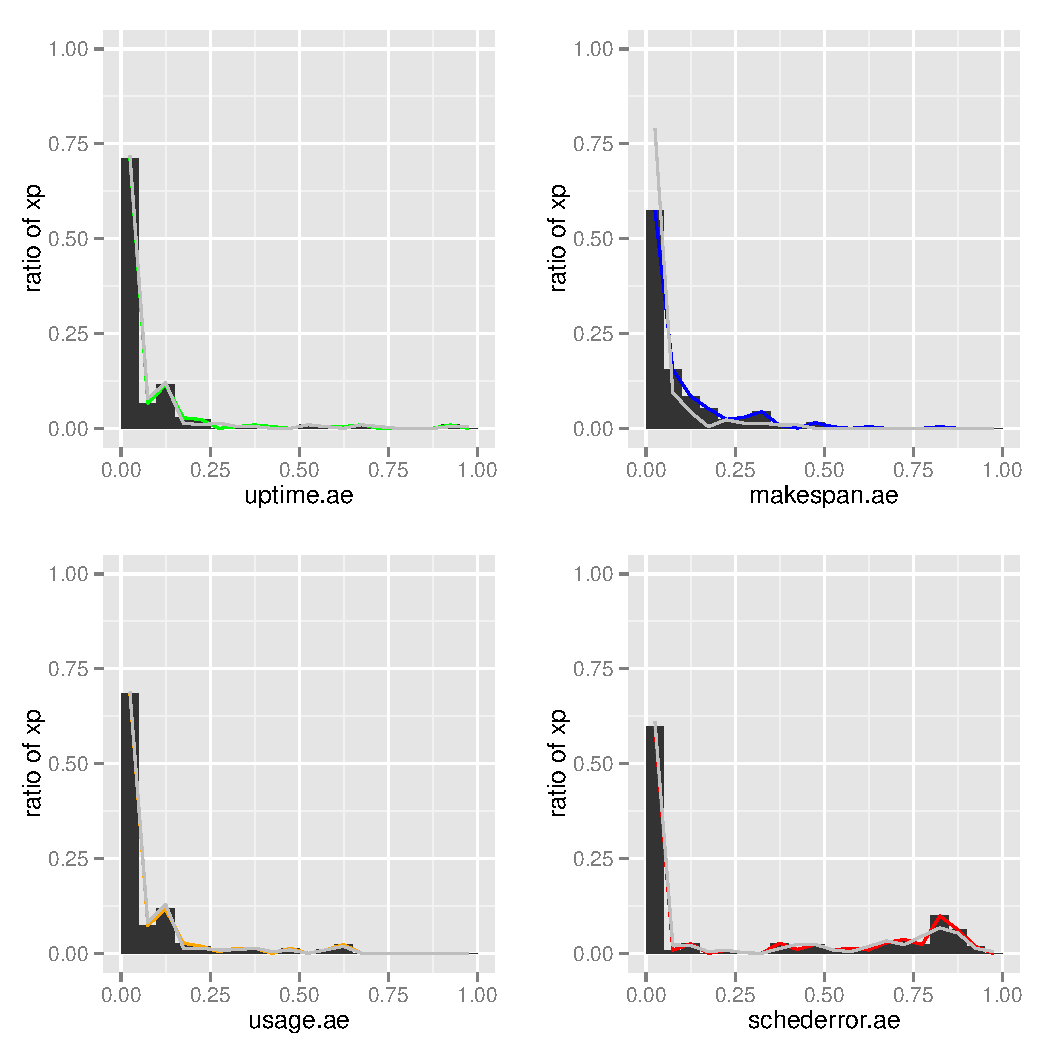
\includegraphics[width=\textwidth]{sim_no-boottimes-4metrics-cmp.pdf}

  \input{\vrpath sim_no-boottimes-4metrics-mmmm.latex}

  \input{\vrpath sim_no-boottimes-4metrics-mmmm-cmp.latex}

  \input{\vrpath sim_no-boottimes-4metrics-mmmm-twobytwo.latex}

  \caption{Frequencies, statistics, and comparison with best of simulations with no real boot times 
  injection}

\end{figure} 

%worst case: v3.standard.2x2.asap.regular.fr-inria.2 
The worst case show a makespan ae of $0.816$ (3141s instead of 17076s). 
This is due to boottimes on BonFire that were completely of charts: 
5 boots were normal (ranging from 232s to 311s), 
the 17 others ranged from 3281s to 11084s.
Whereas BonFire were intended to deliver 22 simultaneous VMs, only 5 were available
at the time of the experiment. Instead of refusing the following 17 VMs, the
provisioning system of BonFire put them in pending state, waiting for the delivered
ones to stop. The VMs being provisioned for one hour, following the 5 normal boots, 
5 boots took approximatively 1 hour, then 5 other boots took 2 hours,
and 5 another more took 3 hours. Finally, 2 boots took 1 hour after the last 
dependencies were satsified.

This illustrates that defective clouds can not be efficiently simulated without 
proper information capture. However, once captured, this kind of defection is
perfectly simulated by SchIaaS. Consequently, it can be used to assess behavior 
and robustness of solutions facing these defections.

%Best case: v3.standard.3x3.afap.regular.de-hlrs.2
Some case are surprisingly improved without the real boot times injection:
For instance, one xp shows a real makespan of 25788s, for 35106s with boot times
injection and 24266s without. 




\subsubsection{No-threads}

Injection of: real boot times and some times due to Schlouder internal threads, 
such as lapses after a node become ready and the start of the first job.

Assess the impact of efficient internal threads simulation

\begin{figure}
  \centering
  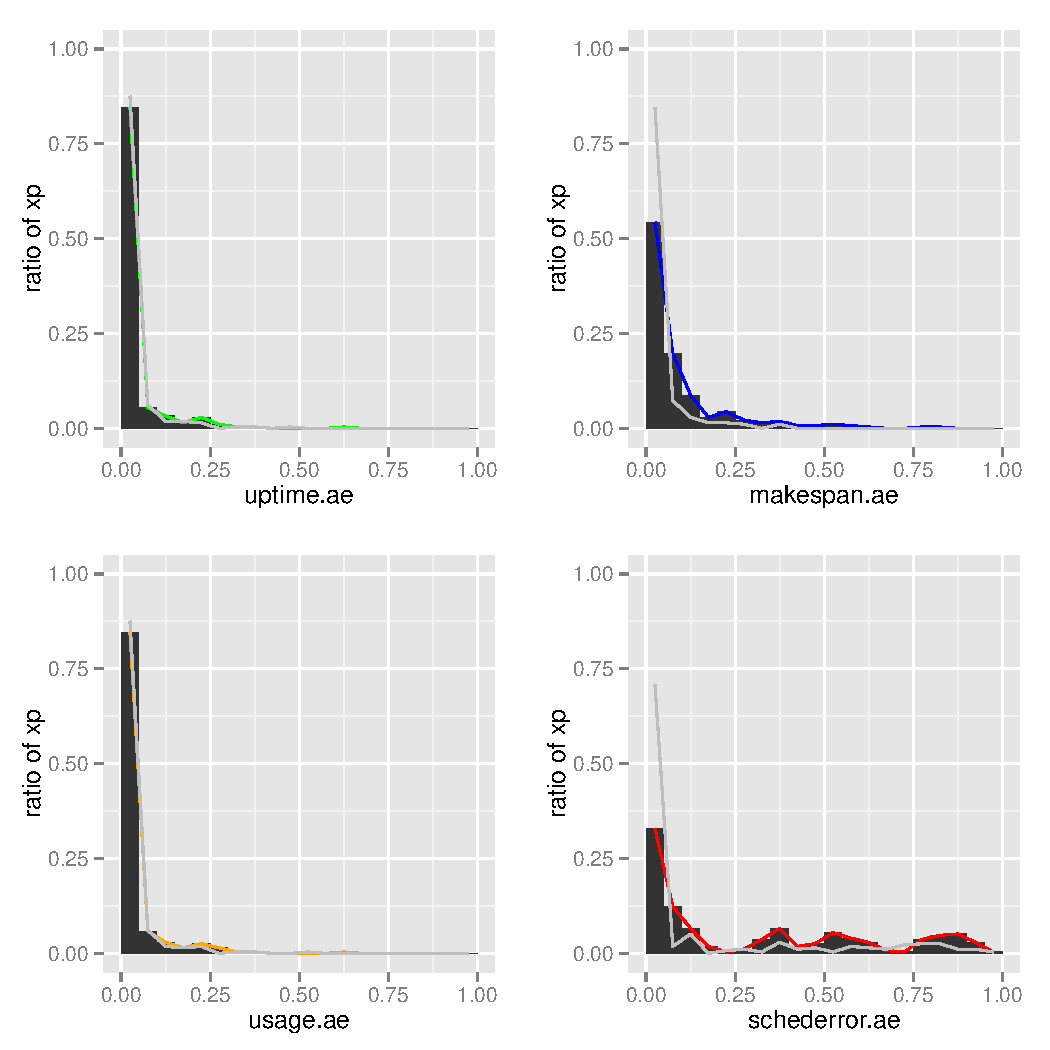
\includegraphics[width=\textwidth]{sim_no-threads-4metrics-cmp.pdf}
  
  \input{\vrpath sim_no-threads-4metrics-mmmm.latex}

  \input{\vrpath sim_no-threads-4metrics-mmmm-cmp.latex}

  \input{\vrpath sim_no-threads-4metrics-mmmm-twobytwo.latex}
    
  \caption{Frequencies, statistics, and comparison with best of simulations with no real thread times
  injection}
\end{figure} 



\subsubsection{Communications}

Injection of: real boot times, some times due to Schlouder internal threads, 
such as lapses after a node become ready and the start of the first job, 
and, real runtimes and real data size for jobs input and output communications.

Assess the impact of efficient communications 

\begin{figure}
  \centering
  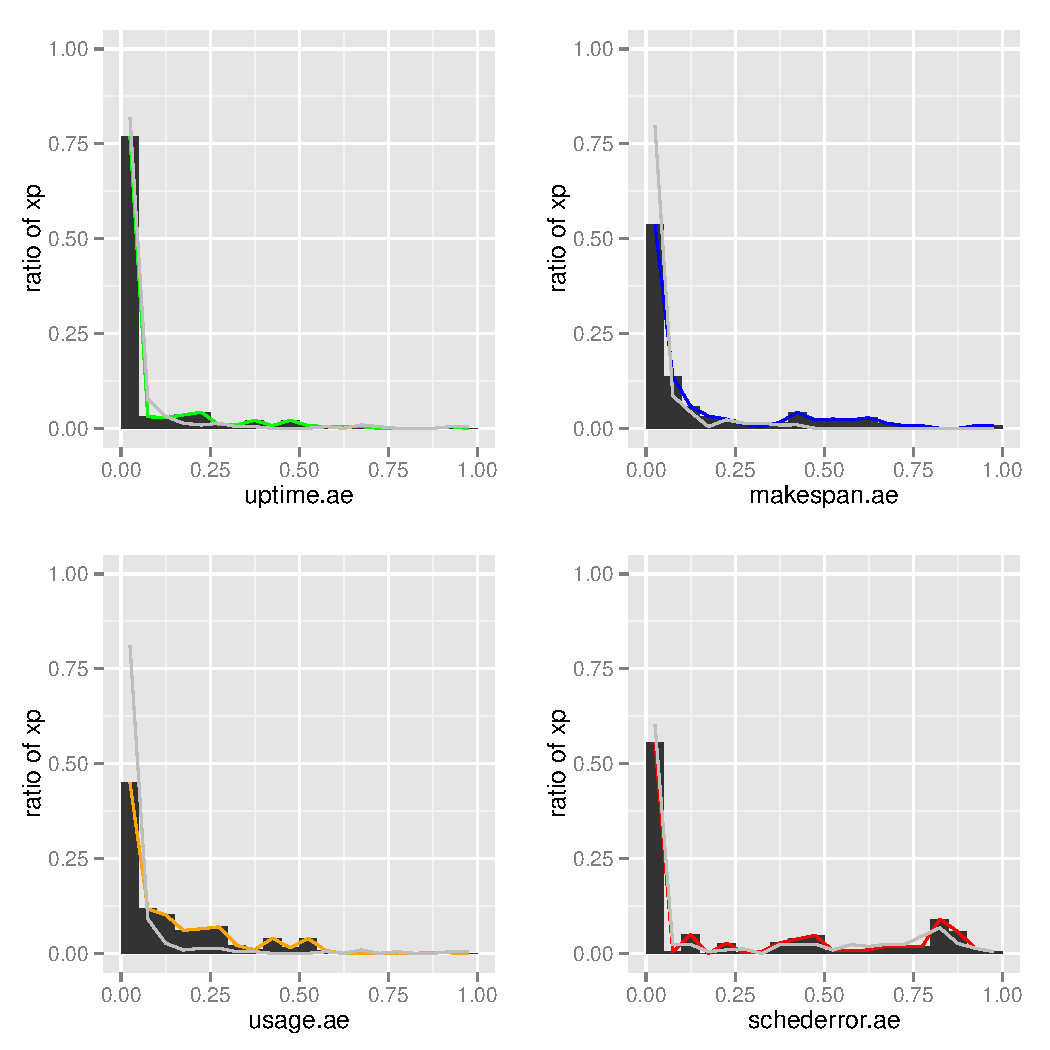
\includegraphics[width=\textwidth]{sim_communications-4metrics-cmp.pdf}
  
  \input{\vrpath sim_communications-4metrics-mmmm.latex}

  \input{\vrpath sim_communications-4metrics-mmmm-cmp.latex}

  \input{\vrpath sim_communications-4metrics-mmmm-twobytwo.latex}

  \caption{Frequencies, statistics, and comparison with best of simulations with simulation of communications}
\end{figure} 

\begin{figure}
  \centering
  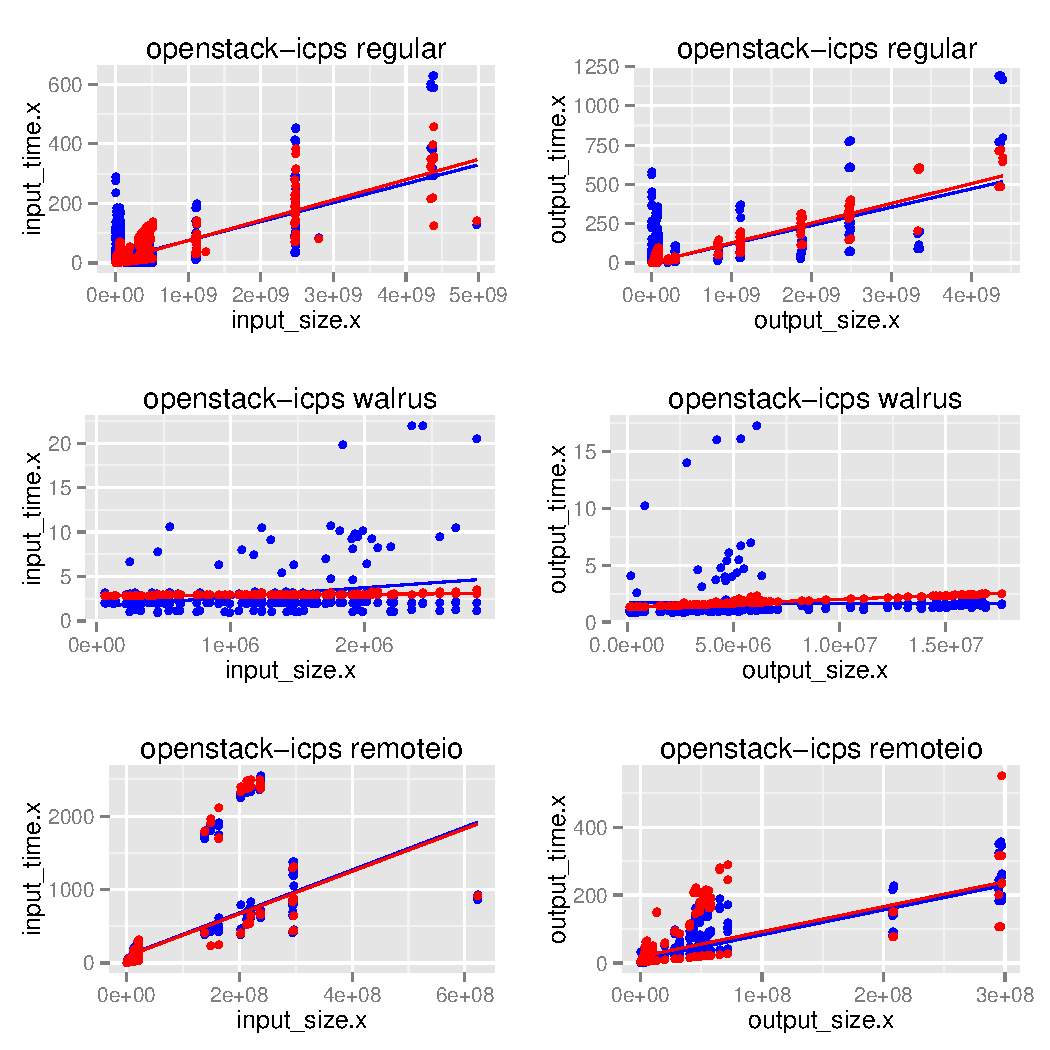
\includegraphics[width=\textwidth]{communications-openstack-icps.pdf}
  
  \caption{Linear regressions of communication times vs. data size, 
    according to platform, storage, and communication direction on openstack-icps}
\end{figure} 


\begin{figure}
  \centering
  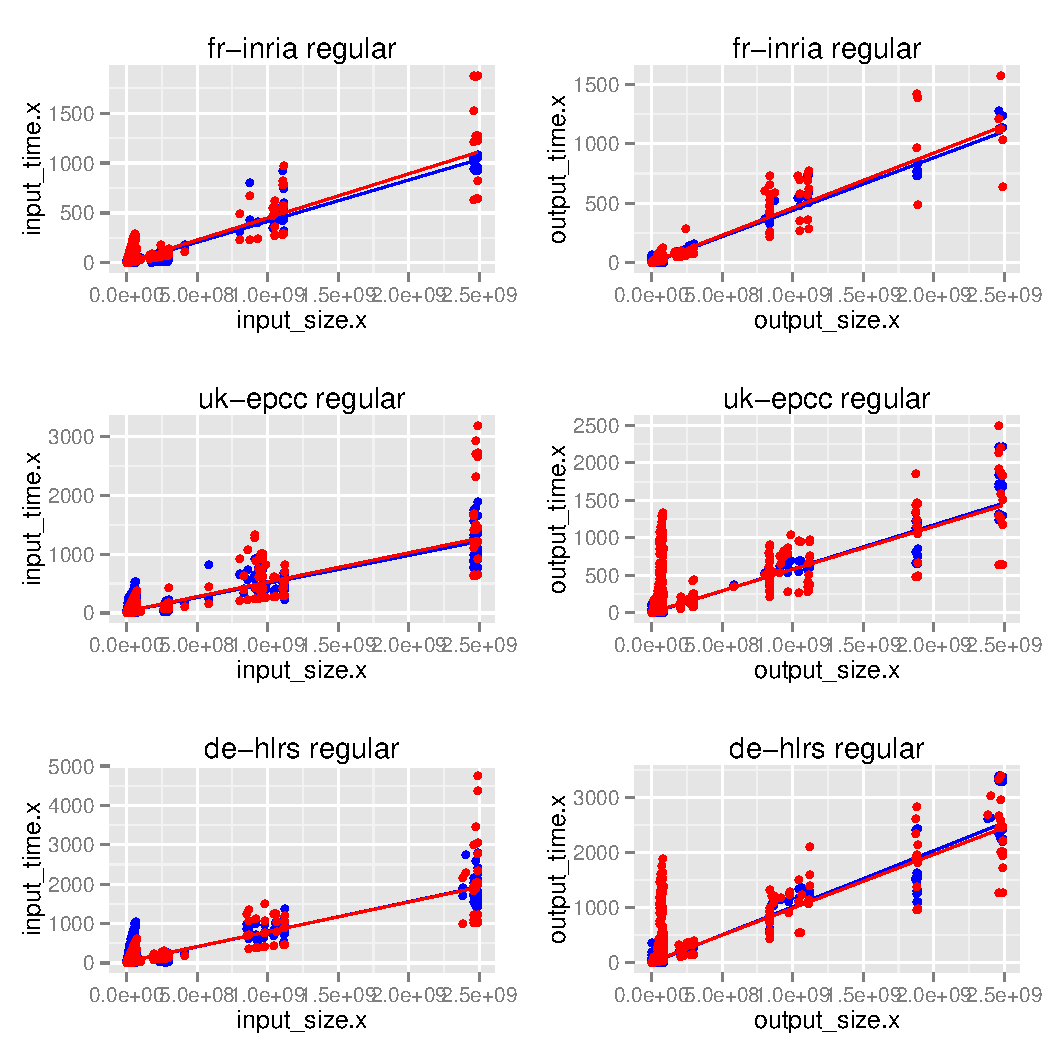
\includegraphics[width=\textwidth]{communications-bonfire.pdf}
  
  \caption{Linear regressions of communication times vs. data size, 
    according to platform, storage, and communication direction on BonFire}
\end{figure} 


\subsubsection{Prediction}

Injection of nothing from the real xp, except the xp description as submitted 
to schlouder.

Assess the efficiency of using a simulator as a predictor of a cloud.

\begin{figure}
  \centering
  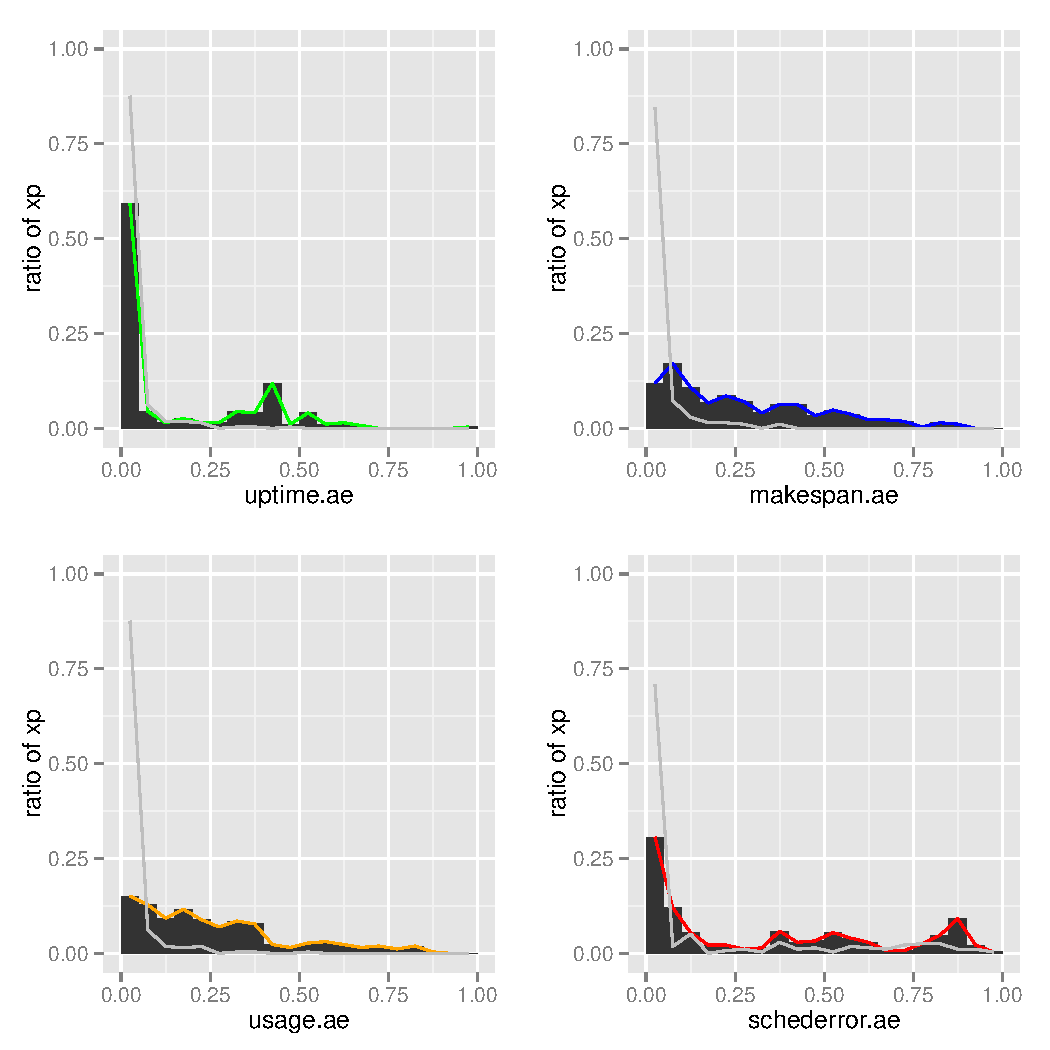
\includegraphics[width=\textwidth]{sim_predictions-4metrics-cmp.pdf}
 
  \input{\vrpath sim_predictions-4metrics-mmmm.latex}
  \input{\vrpath sim_predictions-4metrics-mmmm-cmp.latex}
  \input{\vrpath sim_communications-4metrics-mmmm-twobytwo.latex}

  
  \caption{Frequencies, statistics, and comparison with best of simulations with no injection}
\end{figure} 

\section{Open-science}

\begin{verbatim}
git clone https://git.unistra.fr/gossa/schlouder-traces.git
git clone https://scm.gforge.inria.fr/anonscm/git/schiaas/schiaas.git 
cd schiaas
cmake .
make
cd lab
./lap.py -p2 setup/simschlouder/validation.cfg
cd setup/simschlouder/validation-results
ls
\end{verbatim}





